
\documentclass[conference]{IEEEtran}

\ifCLASSINFOpdf
  \usepackage[pdftex]{graphicx}
  \graphicspath{{../pdf/}{../jpeg/}}
  \DeclareGraphicsExtensions{.pdf,.jpeg,.png}
\else
\fi

\usepackage{pgfplots}
\usepackage{array}
\usepackage{url}
\usepackage[T1]{fontenc}
\usepackage[utf8]{inputenc}

\hyphenation{op-tical net-works semi-conduc-tor}

\begin{document}

\title{A Survey on the Mathematical Emphasis in Brazilian Computer Science Curricula}

\author{\IEEEauthorblockN{Pedro Paulo Vezzá Campos }
\IEEEauthorblockA{Institute of Mathematics and Statistics\\
University of São Paulo\\
São Paulo, Brazil\\
Email: pedrovc@ime.usp.br}
\and
\IEEEauthorblockN{Jackson José Souza}
\IEEEauthorblockA{Institute of Mathematics and Statistics\\
University of São Paulo\\
São Paulo, Brazil\\
Email: jackson@ime.usp.br}
\and
\IEEEauthorblockN{Giuliano Salcas Olguin}
\IEEEauthorblockA{Faculty of Education\\
University of Campinas\\
Campinas, Brazil\\
Email: giuliano.olguin@gmail.com}}

\maketitle


\begin{abstract}
    A recurring question raised by professors and undergraduate students involves the distribution of basic and pratical - or professional - courses. Some authors defend a curriculum with more basic courses, such as Mathematics, Physics and Chemistry, in order to create a solid background. Moreover, there is a growth of academic exchange programs all around the world, which requires a common learning base.

    Since 1960, the importance of Mathematics in Computer Science (CS) undergraduate curricula has been decreasing, particularly, because new fields in CS have risen and they were assimilated in the curricula. Despite of reduction, Mathematics still have its role in CS's curricula.

    The goal of this paper is to analyze the amount of the courses related to Mathematics in different CS undergraduate curricula. In this work are analyzed the lecture hour load dedicated to Mathematics courses on ten Brazilian CS undergraduate programs: The Federal Universities of Ceará, Minas Gerais, Campina Grande, Pernambuco, Rio de Janeiro, Rio Grande do Sul and Santa Catarina, State Universities of São Paulo and Campinas and the Pontifical Catholic University of Rio Grande do Sul. These programs were selected among others due their 5-stars rating in the Guia do Estudante 2012 Ranking, published by Editora Abril.

    To allow this comparison, it was established a definition of what was considered a lecture hour of Mathematics. For a reference point, such programs were compared with two reference curricula in the area: The Brazilian Computer Society (SBC) and the Computer Science Curriculum 2008 made by the IEEE Computer Society and Association for Computing Machinery (ACM) joint task force.

    The curricula presented in the official sites of the selected universities in 2012 were analyzed and it was possible to conclude that more than half of the programs don't achieve the minimum amount of Mathematics study hours necessary during undergraduate studies according to IEEE/ACM's reference curriculum.
\end{abstract}

\IEEEpeerreviewmaketitle

\section{Introduction}
	The recent growth of different courses of higher education have resulted in a worsening of the identity crisis inside the University. Since its creation in the late thirteenth century \cite{oliveira:origem_universidades}, its function varied with the political context of local society, presenting basically values related to national issues. Still, persisted the existence of two orthogonal trends, the one which states that the University's mission should be to fix the current society problems, and the one which states that its main task is to be a beacon, glimpsing the future. The present difficulty is that we have both kinds of programs: Some that aim immediate employability and some that focus in graduate professionals which may be able to deal with problems that still doesn't exist. Merging these two powers seems to be an impossible task.

	In Renato Janine's view \cite{ribeiro:universidade_vida_atual}, there are certain knowledges which are volatile, usually the technical ones, which should be taught by companies. As he quotes in a free translation, ``it's better that in their formation years, the young deal with what's perennial and, with this, will give him a solid foundation, than with details in constant change. ''

	The university should give the necessary foundations so that after graduated the person may be able to adapt to different standards used by companies in the practice of the profession whose qualification was obtained at the university. Therefore, the university should not bother to teach different types of procedures established in the labor market or teach techniques to deal only with some particular problems of the profession. It should rather prepare students to deal with any problem or types of procedures at any time, whether present or future.

	After all, the procedures may vary not only across firms but also change over time. Thus, the trained professional would not be prepared for the future and could only adapt to companies who could handle some certain problems dominate and only some specific techniques. One can easily notice this fact through the rapid evolution of software, which require a constant learning of their manipulation, generating in some cases a disposal of knowledge previously seen.

	Therefore, it is evident that the theory and fundamentals are essential for this type of formation and can not be \emph{replaced} by just technical or practical knowledge. After all, foundations give the ability to take a given problem and use one approach or reasoning to solve it. This issue has greater impact on technology-intensive programs, such as engineering, these still being governed by entities that control the exercise of the profession.

	One of the common points, located in virtually every courses curricula that deal with technology are the contents of Mathematics. Those, which in most cases have only a basic level of depth, precisely fit the definition that Renato Janine presented for tasks to be developed within the University. According to Anthony Ralston \cite{ralston:do_need_mathematics}, Mathematics develops the mind and `` improves students' learning skills.''

	Moreover, both Ralston and Kelemen et al \cite{kelemen:has_become_math_phobic}, are emphatic in noting that the way Mathematics is offered in undergraduate programs in American universities, more specifically the Bachelor in Computer Science (BCC), influences on student learning.

	An important fact detected by several of the studies analyzed (\cite{ralston:do_need_mathematics}, \cite{tucker:our_curriculum_math_phobic}) is that an analysis of the reference curriculum provided by the IEEE and Association for Computing Machinery (ACM) joint task-force \cite{cs2001} \cite{cs2008} indicates that the role of mathematics has been decreasing gradually since at least the 1960s, although at a lower rate today.

	This scenario is considered bad, because for Computer Science / Software Engineering students, in particular, Mathematics is important because the logical reasoning inherent in any mathematical thinking is very similar to logical thinking necessary in software development \cite{ralston:do_need_mathematics}. In developing and implementing software projects, the graduate needs to develop effective ways to solve computational problems and the amount of mathematics used in daily life of a programmer usually increases when the structures are built using a more formal language. \cite{ralston:do_need_mathematics}

	According to \cite{kelemen:has_become_math_phobic}, ``Computer Science students should be able to model `real world' problems precisely using mathematics and using structures like arrays, linked lists, trees, finite graphs and matrices. They should be able to design and analyze algorithms that transform such structures [\ldots], understand the nature of a mathematical model and relate mathematical models to areas of real problems [\ldots]. Strategies for solving problems such as divide-and-conquer and backtracking are also essential.''

\section{Methodology}
	This paper makes a comparative study of different Brazilian Computer Science programs through a quantitative comparison of the number of lecture hours in the area of Mathematics both in absolute and in relative values to the total hours required for graduation. The main goal is to identify whether the selected courses have more or less emphasis on Mathematics compared with two reference curricula in the area, the Brazilian Computer Society (SBC) \cite{sbc} and the Computer Science Curriculum 2008 made by the IEEE Computer Society and Association for Computing Machinery (ACM) joint task force \cite{cs2008}.

	It is important to point, that a quantitative assessment of the hour load allows an objective classification of studided programs, on the other hand, may be less effective in analyzing the different facets that Mathematics is presented in CS undergraduate courses, such as the emphasis of a particular program in the area of Continuous (Calculus) or Discrete Mathematics (Algebra).

% Preamble: \pgfplotsset{width=7cm,compat=1.3}
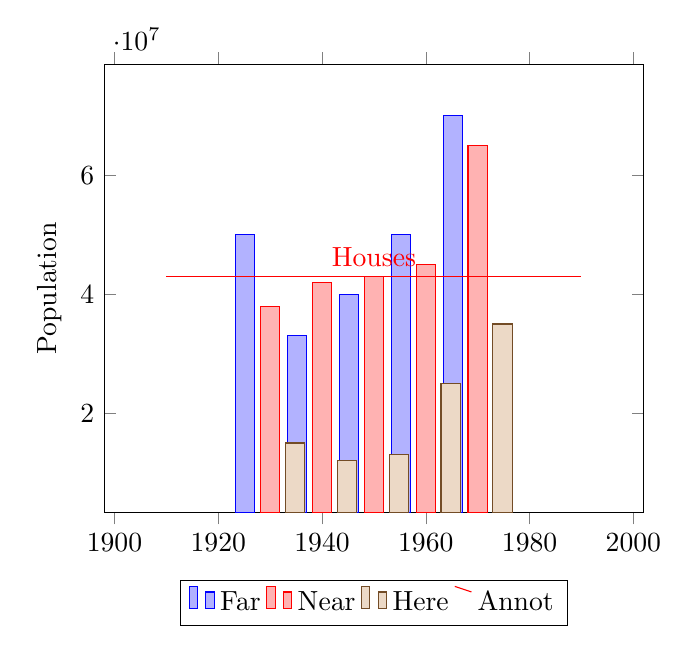
\begin{tikzpicture}
\begin{axis}[
	x tick label style={
		/pgf/number format/1000 sep=},
	ylabel=Population,
	enlargelimits=0.15,
	legend style={at={(0.5,-0.15)},
		anchor=north,legend columns=-1},
	ybar,
	bar width=7pt,
]
\addplot
	coordinates {(1930,50e6) (1940,33e6)
		(1950,40e6) (1960,50e6) (1970,70e6)};
\addplot
	coordinates {(1930,38e6) (1940,42e6)
		(1950,43e6) (1960,45e6) (1970,65e6)};
\addplot
	coordinates {(1930,15e6) (1940,12e6)
		(1950,13e6) (1960,25e6) (1970,35e6)};
\addplot[red,sharp plot,]
	coordinates {(1910,4.3e7) (1990,4.3e7)}
	node[above] at (axis cs:1950,4.3e7) {Houses};
\legend{Far,Near,Here,Annot}
\end{axis}
\end{tikzpicture}

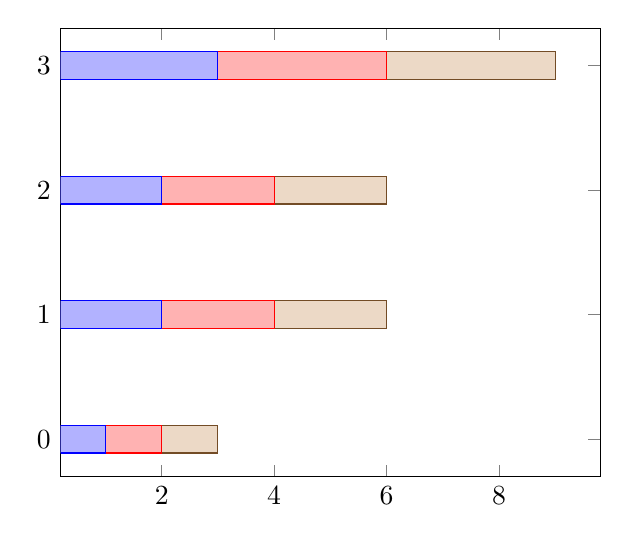
\begin{tikzpicture}
\begin{axis}[xbar stacked]
\addplot
	coordinates {(1,0) (2,1) (2,2) (3,3)};
\addplot
	coordinates {(1,0) (2,1) (2,2) (3,3)};
\addplot
	coordinates {(1,0) (2,1) (2,2) (3,3)};
\end{axis}
\end{tikzpicture}

	For this paper, are considered Math disciplines those that address the areas of Calculus, Linear Algebra, Vectors, Geometry and Algebra. These subjects are usually taught by the Universities Mathematics departments. A difficulty is that in some cases the names of the courses, or their syllabi, do not represent what is actually taught. All curricular material was read and classifications were created to select what in fact can be identified as Mathematics.

	The ten Brazilian CS undergraduate programs studied were selected among other due to their 5-stars rating according to the Guia do Estudante 2012 Ranking, published by Editora Abril. \cite{guia_estudante} The list comprehends the Federal Universities of Ceará (UFC), Minas Gerais (UFMG), Campina Grande (UFCG), Pernambuco (UFPE), Rio de Janeiro (UFRJ), Rio Grande do Sul (UFRGS) and Santa Catarina (UFSC), State Universities of São Paulo (USP) and Campinas (UNICAMP) and the Pontifical Catholic University of Rio Grande do Sul (PUC-RS). USP is further sub-divided in two distinct CS programs, the one held at the Institute of Mathematics and Statistics (IME/USP) and the other held at the Institute of Mathematical Sciences and Computing (ICMC/USP).
	
	A side effect of this choice is that most of the programs studied are held by public universities, which must be taken into account in the data analysis since they may have different emphases in the quantity and approach in fundamentals disciplines (especially Mathematics) in comparison to private universities.
	
\section{Data}
Table 1 presents the general panorama of the 10 universities indicating their size and course characteristics.

\begin{table*}
	\centering
	\caption{Studied CS programs panorama}
    \begin{tabular}{|c|c|c|c|c|c|}
        \hline
        University         & Total credits  & Total hours & Period           & Graduation (years) & Students per year \\ \hline
        IME/USP \cite{ime} & 199            & 2985        & Diurnal           & 4               & 50                   \\ 
        PUC-RS \cite{pucrs}& ....           & ....        & Nocturnal           & 4               & 60                   \\ 
        UFC \cite{ufc}     & ...            & ....        & ... & ...               & ..                   \\ 
        UFCG \cite{ufcg}   & 208            & 3120        & Diurnal           & 4               & 90                   \\ 
        UFMG \cite{ufmg}   & 175            & 2625        & Diurnal           & 4               & 80                   \\ 
        UFPE \cite{ufpe}   & 233            & 3495        & Diurnal           & 4.5             & 100                  \\ 
        UFRGS \cite{ufrgs} & 196            & 3240        & Diurnal           & 4.5             & 100                  \\ 
        UFRJ \cite{ufrj}   & 195            & 3075        & Diurnal           & 4.5             & 50                   \\ 
        UFSC \cite{ufsc}   & 196            & 3528        & Diurnal           & 4               & 100                  \\ 
        UNICAMP \cite{unicamp}& 200         & 3000        & Nocturnal          & 5               & 50                   \\ 
        ICMC/USP \cite{icmc}& 293           & 4395        & Diurnal           & 5               & 100                  \\ 
        SBC \cite{sbc}     & 160            & 2400        & N/A              & 4               & N/A                  \\ 
        SBC \cite{sbc}     & 200            & 3000        & N/A              & 5               & N/A                  \\ 
        ACM \cite{cs2008}  & 280            & 4200        & N/A              & 4               & N/A                  \\
        \hline
    \end{tabular}
\end{table*}

	Nota-se que a maioria dos cursos são Diurnals (Integrais), com duração entre 4 e 4,5 anos. É importante notar que a relação entre um crédito e as respectivas horas de aula varia entre universidades. Há cursos como os da da USP e o currículo de referência da ACM que consideram que um crédito equivale a 15 horas de aula, já o da UFSC, por exemplo, adota a relação 1 crédito = 18 horas. O currículo referência da SBC não indica qual é a relação adotada e assim os autores optaram por considerar o valor de 15 horas para fins de comparação.

	Na composição dos totais apresentados na tabela acima foram descritas as quantidades mínimas necessárias para a integralização curricular completa, abarcando créditos de disciplinas optativas e/ou estágios obrigatórios quando existem. 

	Analisando a coluna de total de horas podemos perceber que há uma grande variabilidade na quantidade exigida pelos currículos das diferentes universidades. Em média são exigidas 3177 h ($\sigma = 554 h $) para cursos de 4 anos, 3270 horas ($\sigma = 211 h$) para cursos de 4,5 anos e 3465 h ($\sigma = **** h$) para cursos de 5 anos.

	A tabela 2 trata especificamente dos conteúdos de Matemática. Aqui percebe-se uma grande diversidade na carga horária reservada a Matemática nos currículos dos cursos de Computação pelo Brasil. Aqui, as universidades possuem em média 15,6\% ($\sigma = 4,77 \%$) de disciplinas exclusivamente de desta área.

	Ainda, notamos que ao compararmos cada universidade com o currículo de referência da ACM (Que afirma ser o mínimo necessário para a cobertura do tópico) podemos verificar que 5 cursos possuem carga de Matemática maior ou igual que o recomendado e 6 cursos possuem menos. Isso corrobora a visão dos autores citados anteriormente que afirmam que Matemática é uma disciplina em decadência nos cursos de Computação.

\begin{table}
	\centering
	\caption{Some Typical Commands}
    \begin{tabular}{|p{2cm}|p{2cm}|p{2cm}|}
        \hline
        Universidade & Créditos Totais em Matemática       & Créditos Percentuais em Matemática        \\ \hline
        IME/USP      & 50                                  & 25,10\%                                   \\ 
        UNICAMP      & 35                                  & 17,40\%                                   \\ 
        UFMG         & 19                                  & 10,80\%                                   \\ 
        UFRGS        & 24                                  & 12,00\%                                   \\ 
        UFRJ         & 31                                  & 21,20\%                                   \\ 
        PUC-RJ       & 22                                  & 10,20\%                                   \\ 
        ICMC/USP     & 36                                  & 16,50\%                                   \\ 
        UFPE         & 25                                  & 10,70\%                                   \\ 
        UFBA         & 32                                  & 16,20\%                                   \\ 
        UFSC         & 21                                  & 12,20\%                                   \\ 
        UFCG         & 28                                  & 13,40\%                                   \\ 
        SBC (4 anos) & 30                                  & 5,30\%                                    \\ 
        ACM          & 43                                  & 15,30\%                                   \\
        \hline
    \end{tabular}
\end{table}

\section{Conclusões}
	Neste artigo foi possível ver primeiramente como as disciplinas de Matemática são de grande importância para um futuro bacharel em Ciência da Computação. Foi visto que tal disciplina é uma base, que precisa ser sólida, para o desenvolvimento de tópicos mais avançados que se baseiam nela. Ainda, diversos educadores na área de Computação com artigos publicados em eventos de repercussão internacional compartilham desta tese.
	
	Por outro lado, foi constatado que esta área está sofrendo uma decadência em sua relevância, em parte pelo surgimento de diversas novas tendências no mercado de Computação que são absorvidas nos currículos dos cursos de graduação.
	
	Por fim, foi feita uma análise da situação atual da ênfase dada a Matemática nos currículos de 11 universidades brasileiras através de análises da carga horária absoluta e relativa. Foi constatado que mais de 50\% das universidades pesquisadas possuem uma carga menor que o recomendado pela ACM em seu currículo de referência.

% An example of a floating figure using the graphicx package.
% Note that \label must occur AFTER (or within) \caption.
% For figures, \caption should occur after the \includegraphics.
% Note that IEEEtran v1.7 and later has special internal code that
% is designed to preserve the operation of \label within \caption
% even when the captionsoff option is in effect. However, because
% of issues like this, it may be the safest practice to put all your
% \label just after \caption rather than within \caption{}.
%
% Reminder: the "draftcls" or "draftclsnofoot", not "draft", class
% option should be used if it is desired that the figures are to be
% displayed while in draft mode.
%
%\begin{figure}[!t]
%\centering
%\includegraphics[width=2.5in]{myfigure}
% where an .eps filename suffix will be assumed under latex, 
% and a .pdf suffix will be assumed for pdflatex; or what has been declared
% via \DeclareGraphicsExtensions.
%\caption{Simulation Results}
%\label{fig_sim}
%\end{figure}

% Note that IEEE typically puts floats only at the top, even when this
% results in a large percentage of a column being occupied by floats.


% An example of a double column floating figure using two subfigures.
% (The subfig.sty package must be loaded for this to work.)
% The subfigure \label commands are set within each subfloat command, the
% \label for the overall figure must come after \caption.
% \hfil must be used as a separator to get equal spacing.
% The subfigure.sty package works much the same way, except \subfigure is
% used instead of \subfloat.
%
%\begin{figure*}[!t]
%\centerline{\subfloat[Case I]\includegraphics[width=2.5in]{subfigcase1}%
%\label{fig_first_case}}
%\hfil
%\subfloat[Case II]{\includegraphics[width=2.5in]{subfigcase2}%
%\label{fig_second_case}}}
%\caption{Simulation results}
%\label{fig_sim}
%\end{figure*}
%
% Note that often IEEE papers with subfigures do not employ subfigure
% captions (using the optional argument to \subfloat), but instead will
% reference/describe all of them (a), (b), etc., within the main caption.


% An example of a floating table. Note that, for IEEE style tables, the 
% \caption command should come BEFORE the table. Table text will default to
% \footnotesize as IEEE normally uses this smaller font for tables.
% The \label must come after \caption as always.
%
%\begin{table}[!t]
%% increase table row spacing, adjust to taste
%\renewcommand{\arraystretch}{1.3}
% if using array.sty, it might be a good idea to tweak the value of
% \extrarowheight as needed to properly center the text within the cells
%\caption{An Example of a Table}
%\label{table_example}
%\centering
%% Some packages, such as MDW tools, offer better commands for making tables
%% than the plain LaTeX2e tabular which is used here.
%\begin{tabular}{|c||c|}
%\hline
%One & Two\\
%\hline
%Three & Four\\
%\hline
%\end{tabular}
%\end{table}




% trigger a \newpage just before the given reference
% number - used to balance the columns on the last page
% adjust value as needed - may need to be readjusted if
% the document is modified later
%\IEEEtriggeratref{8}
% The "triggered" command can be changed if desired:
%\IEEEtriggercmd{\enlargethispage{-5in}}

\bibliographystyle{IEEEtran}
\bibliography{bibliography}


\end{document}

